% The probability that the key i is on the search path for x in a random
% binary search tree on 0..n-1: (a) x a key, (b) x between two keys
% (Morin, figure 7.4). Build: make figures (in ../build).
\documentclass[border=4pt]{standalone}
\usepackage[T1]{fontenc}
\usepackage{lmodern}
\usepackage{amsmath,amssymb}
\usepackage{tikz}
\usepackage{lamalunga}
% tikz-ads.tex: the TikZ styles shared by the figures of the memory of the
% manual, \input by each standalone figure: a cell of a vector (cell), the
% cell that an operation touches (touched), a free cell (free), a node of a
% linked structure (node), the labels of indices (index) and of variables
% (var), a pointer (ptr), and \cells and \indices to draw a row of cells.
\usetikzlibrary{arrows.meta,positioning,calc,fit,shapes.multipart}
\definecolor{adsTouched}{RGB}{214,196,236}
\definecolor{adsFree}{RGB}{236,236,236}
\tikzset{
  ads/.style={>={Stealth[length=2mm]},font=\small,
              every node/.append style={inner sep=0pt}},
  cell/.style={draw,minimum width=7mm,minimum height=7mm,
               font=\small\ttfamily,outer sep=0pt},
  touched/.style={cell,fill=adsTouched},
  free/.style={cell,fill=adsFree,text=black!45},
  node/.style={draw,rounded corners=1pt,minimum width=8mm,
               minimum height=6mm,font=\small\ttfamily},
  index/.style={font=\scriptsize\ttfamily,text=black!60},
  var/.style={font=\small\itshape},
  ptr/.style={->,thick}
}
% \cells{name}{x,y}{list}: a row of cells, the first at (x,y), named
% name-0, name-1, ...; each item is text/style, the style one of cell,
% touched and free (e.g., {a/cell,e/touched,/free})
\newcommand{\cells}[3]{%
  \foreach \v/\s [count=\i from 0] in {#3}
    \node[\s] (#1-\i) at ($(#2)+(\i*7mm,0)$) {\v};}
% \indices{name}{n}: the indices 0 .. n-1 under the cells of name
\newcommand{\indices}[2]{%
  \foreach \i in {0,...,\numexpr#2-1\relax}
    \node[index,below=1.2mm of #1-\i] {\i};}

\begin{document}
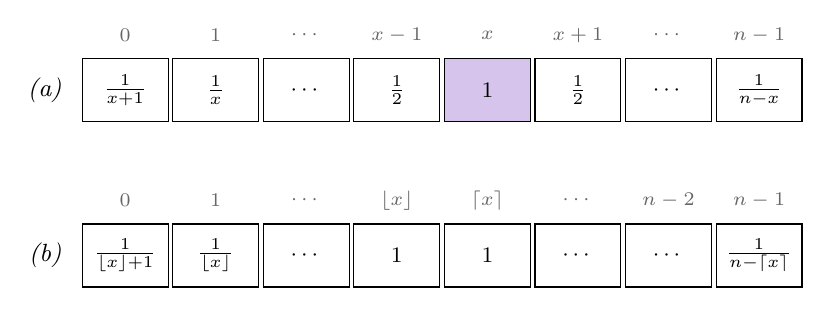
\begin{tikzpicture}[ads]
  \node[index] at (0mm,7mm) {$0$};
  \node[index] at (11.5mm,7mm) {$1$};
  \node[index] at (23mm,7mm) {$\cdots$};
  \node[index] at (34.5mm,7mm) {$x-1$};
  \node[index] at (46mm,7mm) {$x$};
  \node[index] at (57.5mm,7mm) {$x+1$};
  \node[index] at (69mm,7mm) {$\cdots$};
  \node[index] at (80.5mm,7mm) {$n-1$};
  \node[cell,minimum width=10.9mm,minimum height=8mm,font=\footnotesize] (a0) at (0mm,0mm) {$\frac{1}{x+1}$};
  \node[cell,minimum width=10.9mm,minimum height=8mm,font=\footnotesize] (a1) at (11.5mm,0mm) {$\frac{1}{x}$};
  \node[cell,minimum width=10.9mm,minimum height=8mm,font=\footnotesize] (a2) at (23mm,0mm) {$\cdots$};
  \node[cell,minimum width=10.9mm,minimum height=8mm,font=\footnotesize] (a3) at (34.5mm,0mm) {$\frac{1}{2}$};
  \node[touched,minimum width=10.9mm,minimum height=8mm,font=\footnotesize] (a4) at (46mm,0mm) {$1$};
  \node[cell,minimum width=10.9mm,minimum height=8mm,font=\footnotesize] (a5) at (57.5mm,0mm) {$\frac{1}{2}$};
  \node[cell,minimum width=10.9mm,minimum height=8mm,font=\footnotesize] (a6) at (69mm,0mm) {$\cdots$};
  \node[cell,minimum width=10.9mm,minimum height=8mm,font=\footnotesize] (a7) at (80.5mm,0mm) {$\frac{1}{n-x}$};
  \node[var,anchor=east] at (-8mm,0) {(a)};
  \node[index] at (0mm,-14mm) {$0$};
  \node[index] at (11.5mm,-14mm) {$1$};
  \node[index] at (23mm,-14mm) {$\cdots$};
  \node[index] at (34.5mm,-14mm) {$\lfloor x\rfloor$};
  \node[index] at (46mm,-14mm) {$\lceil x\rceil$};
  \node[index] at (57.5mm,-14mm) {$\cdots$};
  \node[index] at (69mm,-14mm) {$n-2$};
  \node[index] at (80.5mm,-14mm) {$n-1$};
  \node[cell,minimum width=10.9mm,minimum height=8mm,font=\footnotesize] (b0) at (0mm,-21mm) {$\frac{1}{\lfloor x\rfloor+1}$};
  \node[cell,minimum width=10.9mm,minimum height=8mm,font=\footnotesize] (b1) at (11.5mm,-21mm) {$\frac{1}{\lfloor x\rfloor}$};
  \node[cell,minimum width=10.9mm,minimum height=8mm,font=\footnotesize] (b2) at (23mm,-21mm) {$\cdots$};
  \node[cell,minimum width=10.9mm,minimum height=8mm,font=\footnotesize] (b3) at (34.5mm,-21mm) {$1$};
  \node[cell,minimum width=10.9mm,minimum height=8mm,font=\footnotesize] (b4) at (46mm,-21mm) {$1$};
  \node[cell,minimum width=10.9mm,minimum height=8mm,font=\footnotesize] (b5) at (57.5mm,-21mm) {$\cdots$};
  \node[cell,minimum width=10.9mm,minimum height=8mm,font=\footnotesize] (b6) at (69mm,-21mm) {$\cdots$};
  \node[cell,minimum width=10.9mm,minimum height=8mm,font=\footnotesize] (b7) at (80.5mm,-21mm) {$\frac{1}{n-\lceil x\rceil}$};
  \node[var,anchor=east] at (-8mm,-21mm) {(b)};
\end{tikzpicture}
\end{document}
